\section{\acf{SDL}}
\label{sc:SDL}
Die \ac{SDL} (\ac{SDL}, engl. Spezifikations und Beschreibungssprache) ist eine von der \ac{ITU-T} (\ac{ITU-T}, engl. Internationalen 
Telekommunikations- Vereinigung für Standardisierung der Telekommunikation) standardisierte objektorientierte Modellierungssprache und wurde erstmalig 
1976 definiert. Die aktuellste Version von \ac{SDL} ist \ac{SDL}-2010, welche eine Überarbeitung der \ac{SDL}-Version \ac{SDL}-2000 aus dem Jahre 
1999 ist. Wenn im folgenden von \ac{SDL} gesprochen wird, wird immer die Version \acs{SDL}-2010 gemeint. 
In den letzten Überarbeitungen wurde die Definition von \ac{SDL} um objekt-orientierte Aspekte erweitert und mit Sprachen wie \ac{UML} und \ac{ASN1} harmonisiert.
\ac{SDL} wird zur Beschreibung von Telekommunikationssystemen, deren Abläufe, sowie für Protokoll Definitionen und in verteilten Systemen eingesetzt.
Der Anwendungsbereich erstreckt sich über komplexe ereignisgesteuerte, interaktiven Echtzeitanwendungen, welche über Nachrichten miteinander kommunizieren. 
Der Hauptfokus von \ac{SDL} ist, sich einen genauen Überblick über das Verhalten genannter Systeme zu machen, wobei Eigenschaften mit anderen Techniken beschrieben werden müssen. 
So wird \ac{MSC} unter anderem zum Beschreiben von Interaktionsverhalten zwischen Systemen, \ac{ASN1} für die Beschreibung von Datentypen und \ac{TTCN3} für Tests verwendet.


\subsection{Architektur}
\label{ssc:Architektur}
Die \ac{SDL}-Spezifikation erlaubt die strukturierte Trennung in Diagramme und Pakete und somit ein aufteilen eines Systems in viele kleinere Teilsysteme,
wodurch die Entwicklung in größeren Gruppen vereinfacht wird.
Dies führt zu dazu, dass andere Sprachen in Pakete definiert werden können und so eine Erweiterung der \ac{SDL}-Spezifikation andere Sprachdefinitionen möglich ist.
Die Struktur ist hierarchisch gegliedert und besteht aus Prozessen, die logisch in Blöcke unterteilt werden können.
Prozesse sind durch untereinander kommunizierende endliche Automaten dargestellt, welche abstrakte Datentypen und Merkmale von Objektorientierung besitzen.
Die Blöcke können in sich selbst gegliedert werden und bilden einzeln oder zusammen dann die höchste Ebene, das System. Diese Struktur wird anhand folgender Abbildung \ref{fig:ArchModell} veranschaulicht.
 
\begin{figure}[ht]
	\centering
	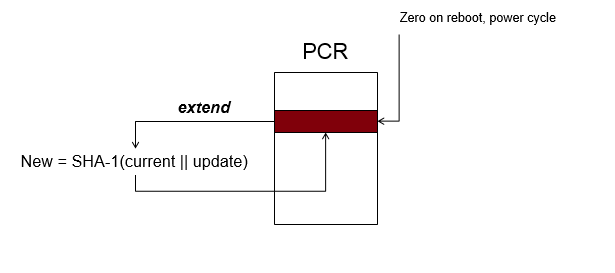
\includegraphics[width=1\textwidth]{test.png}
	\caption{Architekturmodell}
	\label{fig:ArchModell}
\end{figure}

\subsubsection{Agenten}
Wie in Abbildung \ref{fig:ArchModell} zu sehen ist, wird die Struktur der Sprachdefinition durch sogenannte Agenten beschrieben.
Das System ist in der Hierarchie der oberste Agent und kann eine Menge an Agenten enthalten jedoch selbst nicht in einem Agenten beinhaltet sein.
Alles Außerhalb des Systems wird als Umgebung bezeichnet. Blöcke sind Container für Agenten, wodurch die Komplexität und die Größe von Systemen partitioniert wird.
Das System selbst ist ein Block, welcher als Container für Blöcke verwendet wird. 
Prozesse sind Agenten der untersten Ebene, sind innerhalb von Blöcken, können keine weiteren Agenten enthalten und bestehen aus \ac{EFSM}s.


\subsection{Kommunikation}
\label{ssc:Kommunikation}
Die Kommunikation innerhalb von \ac{SDL} findet entweder asynchron über Nachrichten oder mit diskreten Signalen über Kanäle statt. 
Diese können sowohl auf Systemebene, als auch auf Blockebene definiert werden.
Jede Nachricht besitzt einen Namen, optionale Parameter und kann in eine Liste gruppiert werden. 
Die Kanäle enthalten ebenfalls Namen und verbinden die einzelnen Agenten untereinander oder mit der Umgebung.
Ein Kanal besteht immer aus einer Quelle und einem Endpunkt, welche Bi- oder Unidirektional definiert werden können. Der Kanal muss entweder in einem Prozess oder in die Umgebung enden.
 Abbildung \ref{fig:KommModell} verdeutlicht dies in einem Beispiel.
 
\begin{figure}[ht]
	\centering
	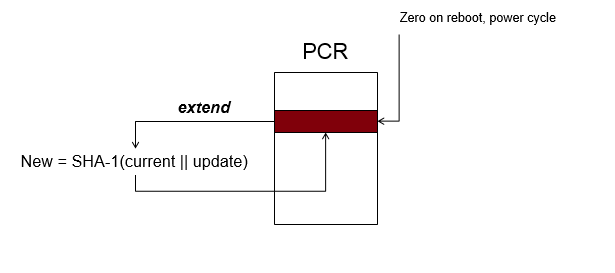
\includegraphics[width=1\textwidth]{test.png}
	\caption{Kommunikationsmodell}
	\label{fig:KommModell}
\end{figure}

Wie in der Abbildung zu sehen ist...(Abbildung beschreiben)


\subsection{Verhalten}
\label{ssc:Verhalten}
Das Verhalten von \ac{SDL} wird in Prozessen definiert, welche wie eben besprochen, durch \ac{EFSM}s repräsentiert werden. Sie bestehen aus einer Menge an Zustandsübergängen, welche Beispielhaft in Abbildung \ref{fig:BspProzess} zu sehen sind. Darunter gehören Zustände wie [liste aufzählen]. Da eine Aufzählung den Rahmen sprengen würde, ist die Vollständige Liste aus der Spezifikation zu entnehmen. 
Die Modellierung der Automaten richtet sich nach Mealy, wobei in diesem die Ausgabe von seinem Zustand und seiner Eingabe abhängt.
Im Gegensatz zu Moore-Automaten enthält er keinen Startzustand, wobei jeder Mealy-Automat in einen Moore-Automat übertragen werden kann.
Diese Automaten können Operationen an Daten vornehmen und kommunizieren über Nachrichten welche am Endpunkt des Kanals gelistet sind. Prozesse besitzen eine \ac{FIFO}-Eingabeschlange, welche der Prozess nach und nach abarbeitet. Kommen 2 Nachrichten gleichzeitig an, so ist es zufällig, welche der beiden Nachrichten zuerst ausgeführt wird. 

\subsubsection{Zustände}
\label{sssc:Verhalten}

\begin{figure}[ht]
	\centering
	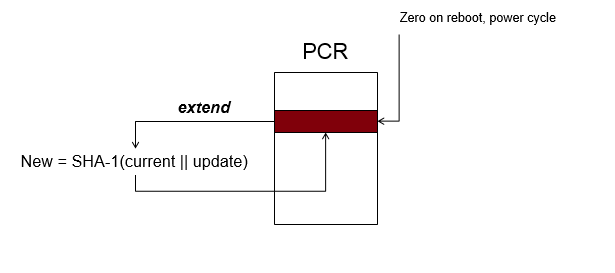
\includegraphics[width=1\textwidth]{test.png}
	\caption{Beispiel Prozess}
	\label{fig:BspProzess}
\end{figure}

Wie in der Abbildung zu sehen ist...(Abbildung beschreiben)

\subsection{Daten}
\label{ssc:Daten}
In \ac{SDL} sind Daten auf zwei Arten beschrieben, einerseits mit dem \ac{ADT}(abstract data type) oder mit \ac{ASN1}. \ac{ADT} definiert keine 
Datenstrukturen, sondern jeweils einen Satz an Werten, Operation und Bedingungen. In \ac{ADT} sind einige Datentypen wie Boolean oder Integer vordefiniertl. Die vollständige Liste ist in der Spezifikation zu entnehmen [101/4 S.?].  Dadurch können Daten unter Sprachen ausgetauscht werden und bereits bestehende Datenstrukturen wiederverwendet werden. Folgende 
Abbildung x.x veranschaulicht dies an einem Beispiel. \ac{SDL} beschreibt noch einen 
fortgeschrittener Ansatz von \ac{ADT}, wo Operationen unter anderem zum verstecken von 
Datenmanipulation verwendet werden, dies kann bei weiterem Interesse in der Spezifikation 
[Spezifikation eintragen] nachgelesen werden. 


\begin{figure}[ht]
	\centering
	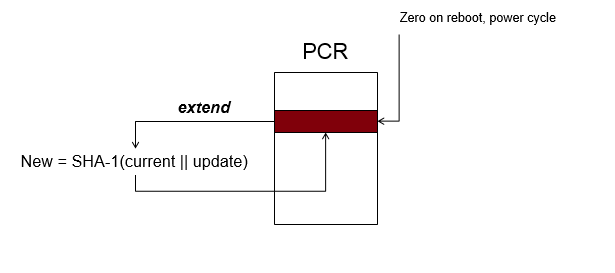
\includegraphics[width=1\textwidth]{test.png}
	\caption{Beispiel Prozess}
	\label{fig:BspProzess}
\end{figure}

Wie in der Abbildung zu sehen ist...(Abbildung beschreiben)
   
\subsection{Objektorientierung} 
\label{ssc:Vererbung}
Die seit


\subsection{Diagramarten}
\label{ssc:Diagramarten}

\subsection{Spracheigenschaften}
\label{ssc:Spracheigenschaften}
Die Eigenschaften der Sprachdefinition von \ac{SDL} sind folgend beschrieben[REC111P.3]:
\begin{itemize}{
		\item[Abstrakte Grammatik] Die abstrakte Grammatik von \ac{SDL} wird von einer abstrakten Syntax und  statischen Bedingungen 
		beschrieben. Die Abstrakte Syntax kann entweder mit einer textbasierten Grammatik oder einem grafischen Metamodell erstellt werden.
		
		\item[Konkrete Grammatik] Die konkrete Syntax wird durch eine grafische Syntax, statischen Bedingungen und Regeln für die grafische Syntax beschrieben.
		Beschrieben wird sie durch die erweiterte Backus-Naur Form. Wenn jedoch in der abstrakten Grammatik ein 
		grafisches Metamodell verwendet wurde, ist es erlaubt dieses um kontrkete Eigenschaften zu erweitert und zu verwenden.
		
		\item[Semantik] Die Semantik beschreibt ein Konstrukt,samt dessen Eigenschaften, Interpretation und dynamischen Bedingungen.
		
		\item[Model] Ein Model gibt Notationen eine Abbildungsform, wenn diese keine direkte abstrakten Syntax besitzen.
}\end{itemize}

\subsubsection{Metamodell}
\label{ssc:Metamodell}
Es werden Anstrengungen unternommen, jedoch existiert derzeit kein öffentlich zugängliches Metamodell von \ac{SDL}, welches alle 
Aspekte der Sprache in sich vereinigt. So hat die \ac{ITU-T} selbst ein Meta-Metamodell auf Grundlage von 
\ac{UML} zu erstellen, jedoch deckt diese Definition, welche auch SDL-UML genannt wird, nur Teile der Sprachdefinition von \ac{SDL} 
ab.
